
\chapter{�����б����ֵ�ѧϰ��������Ķ�ģ̬��������}


\section{Problem Formulation}
\label{subsec:formulation}

Without loss of generality, we assume that there are $M$ data sets $\{\mathbf{X}_1,\mathbf{X}_2,\cdots,\mathbf{X}_M\}$ from different modalities
and each dataset has the same $N$ data samples. Suppose that $\mathbf{X}_m\!=\![\mathbf{x}_{m,1},\mathbf{x}_{m,2},\cdots,\mathbf{x}_{m,N}]\in\!\mathbb{R}^{p_m\times{N}}$
stems from the $m$-th modality, where $p_m$ denotes the dimensionality of the $m$-th modality.
Each data sample pair $\{\mathbf{x}_{1,i},\mathbf{x}_{2,i},\cdots,\mathbf{x}_{M,i} |~\forall i\in [1:N] \}$
exclusively belongs to one of $C$ classes and describes a similar (semantic) concept.

Let $\mathbf{D}_m = [\mathbf{D}_{m(1)},\mathbf{D}_{m(2)},\ldots,\mathbf{D}_{m(C)}] \in \mathbb{R}^{{p_m}\times{K}}$ be the structured discriminative dictionary from $\mathbf{X}_m$ and let $\mathbf{A}_m\in \mathbb{R}^{K \times N}$ be its corresponding sparse coefficients, where $K$ is the size of the dictionary\textcolor{blue}{, and each sub-dictionary $\mathbf{D}_{m(c)} \in \mathbb{R}^{{p_m}\times{(K/C)}}$}. Analogously, $\mathbf{X}_{m(c)}$ is denoted as the data $\mathbf{X}_{m}$ with $c$-th label and $\mathbf{A}_{m(c)}$ is the sparse coefficient corresponding to $\mathbf{X}_{m(c)}$. We also suppose that a common label matrix $\mathbf{Q}=[\mathbf{q}_1,\mathbf{q}_2,\ldots,\mathbf{q}_N]\in\!\{0,1\}^{C\times{N}}$, where $\mathbf{q}_i$ is the label vector of the $i$-th data sample pair. For the $i$-th data sample pair, if it belongs to the $j$-th class, $q_{ij}=1$, otherwise $q_{ij}=0$.
%And one data sample belongs to only one class, \emph{i.e.}, $\sum_{j=1}^C{q_{ij}}=1$ for the $i$-th data sample pair.

Our model aims to separately obtain the sparse coefficients of data from different modalities by dictionary learning, and then project them to the common label space, where the data share the similar semantic concepts by label alignment. On the other
hand, the discriminative dictionary introduced into our model
can ensure the ability of separating different classes, which
is expected to boost the performance of retrieval. Therefore,
the objective function is formulated as the following minimization problem:
\begin{flalign}\label{equ:object}
&\min_{\mathbf{D}_m,\mathbf{A}_m,\mathbf{W}_m} ~\sum\limits_{m=1}^{M} \sum\limits_{c=1}^{C} \big\|\mathbf{X}_{m(c)}-\mathbf{D}_{m(c)} \mathbf{A}_{m(c)}\big\|_{\mathrm{F}}^2  \nonumber \\
& \quad\quad\quad\quad\quad~  +\sum_{m=1}^M  \big\|\mathbf{Q}-\mathbf{W}_m \mathbf{A}_m\big\|_{\mathrm{F}}^2 \nonumber \\
& \quad\quad\quad\quad\quad~  +\sum_{m=1}^M  \lambda_m \|\mathbf{A}_m\|_1 + \sum_{m=1}^M \gamma \|\mathbf{W}_m\|_{\mathrm{F}}^2,
\end{flalign}
where the first term minimizes the reconstruction error, and the the second term aligns the common labels of the same data samples by minimizing the projection error.
It is worth noting that the size of dictionary $K$ is the same for any modalities so that different feature can be projected into a common label space.
The regularization parameters $\lambda_m$ and $\gamma$ can balance the weights of the terms in the objective function.
In Eq.~\eqref{equ:object}, $\mathbf{W}_m\in\mathbb{R}^{C \times K}$ is the projection matrix,
by which $\mathbf{A}_m$ is projected into the common label space.
The term ${\left\| \mathbf{W}_{m} \right\|}_{\mathrm{F}}^2$ is introduced to avoid over-fitting.
In our model, different modalities of input data can be captured and correlated simultaneously.



\section{Optimization Algorithm}
\label{subsec:optimization}

Since the objective function is not jointly convex \textit{w.r.t.} $\mathbf{D}_m$, $\mathbf{A}_m$ and $\mathbf{W}_m$, it is difficult to optimize them jointly. Therefore we use an iterative algorithm to update each one variable when fixing the other two for each modality, alternatively.

We first update $\mathbf{D}_m$. By applying joint dictionary learning, $\mathbf{D}_m$  is calculated for initializing the optimization procedure. To obtain a discriminative dictionary, the Fisher Discrimination Dictionary Learning (FDDL) scheme \cite{yang2011fisher} is applied for the initialization. We consider the sparse coefficients $\mathbf{A}_m$ and mapping matrices $\mathbf{W}_m$ as constants when updating the two dictionaries during each iteration.
Therefore, the dictionary $\mathbf{D}_m$ can be updated through solving the following optimization problem:
\begin{flalign}\label{equ:update-d}
&\min_{\mathbf{D}_{m}} ~\sum\limits_{m\in \mathcal{M}}{\sum\limits_{c=1}^{C}{\big\| {\mathbf{X}_{m(c)}}-{\mathbf{D}_{m(c)}}{\mathbf{A}_{m(c)}} \big\|_{\mathrm{F}}^{2}}} \\
&\mathrm{~s.t.} \quad~\|\mathbf{d}_{m,i}\|_2\leq1, \quad \forall i \nonumber
\end{flalign}
which is essentially a quadratically constrained quadratic programming (QCQP) problem in terms of the target dictionary matrix
$\mathbf{D}_{m(c)}$ \cite{yang2010metaface}.

Next, when the mapping matrix $\mathbf{W}_m$ and dictionary $\mathbf{D}_m$ are fixed,
we can acquire the sparse coefficients in $\mathbf{A}_m$.
As a result, Eq.~\eqref{equ:object} is converted to the following problem:
\begin{flalign}\label{equ:update-a0}
\min_{\mathbf{A}_m}  ~{\big\|\mathbf{X}_m-\mathbf{D}_m \mathbf{A}_m\big\|_{\mathrm{F}}^2 + \big\|\mathbf{Q}-\mathbf{W}_m \mathbf{A}_m\big\|_{\mathrm{F}}^2 +\lambda_m \|\mathbf{A}_m\|_1.  }
\end{flalign}
To conduct the optimization above, the first two terms of Eq.~\eqref{equ:update-a0} can be combined into one term,
leading to the following simplified problem:
\begin{flalign}\label{equ:update-a}
\min_{\mathbf{A}_m}~\big\| \mathbf{\hat{X}}_m - \mathbf{\hat{D}}_m \mathbf{A}_m\big\|_{\mathrm{F}}^2 + \lambda_m \|\mathbf{A}_m\|_1,
\end{flalign}
where $\mathbf{\hat{X}}_{m}=\left[\begin{array}{c} \mathbf{D}_m \\ \mathbf{W}_m \\ \end{array} \right]$
and $\mathbf{\hat{D}}_{m}=\left[\begin{array}{c} \mathbf{X}_m \\ \mathbf{Q} \\ \end{array} \right]$.
Then Eq.~\eqref{equ:update-a} is converted into a standard sparse coding problem,
which can be efficiently solved using the available SPAMS Toolbox \cite{mairal2009online}.

Finally, we try to update the projection matrix $\mathbf{W}_m$.
When $\mathbf{D}_m$ and $\mathbf{A}_m$ are fixed, Eq.~\eqref{equ:object} becomes a ridge regression problem
and its analytical solution can be obtained through solving an easier problem:
\begin{equation}\label{equ:update-w0}
\min_{\mathbf{W}_m} ~{ \big\|\mathbf{Q}-\mathbf{W}_m \mathbf{A}_m\big\|_{\mathrm{F}}^2 + \gamma \|\mathbf{W}_m\|_{\mathrm{F}}^2. }
\end{equation}
It is not difficult to attain the analytical solution to Eq.~\eqref{equ:update-w0} as
\begin{equation}\label{equ:update-w}
\mathbf{W}_m^* = \mathbf{Q} \mathbf{A}_m^\top \big(\mathbf{A}_m \mathbf{A}_m^\top + \gamma \mathbf{I} \big)^{-1}.
\end{equation}

The above procedure iterates until $\mathbf{D}_m$, $\mathbf{A}_m$ and $\mathbf{W}_m$ all converge.
Algorithm \ref{alg:optimization} describes the optimization procedure of our cross-modal learning model.
After the optimization is completed, we can immediately apply our learning model to cross-modal retrieval tasks.

\renewcommand{\algorithmicrequire}{\textbf{Input:}} % Use Input in the format of Algorithm
\renewcommand{\algorithmicensure}{\textbf{Output:}} % Use Output in the format of Algorithm
\renewcommand{\baselinestretch}{1.5}
\begin{algorithm}[!t]
\caption{~~The optimization algorithm for our proposed cross-modal learning model. }
\label{alg:optimization}
\begin{algorithmic}[1]
\Require
Data matrices $\{\mathbf{X}_m\}_{m=1}^M$ with $M$ different modalities and a common label matrix $\mathbf{Q}$.
\Ensure
Dictionaries $\{\mathbf{D}_m\}_{m=1}^M$ and mapping matrices $\{\mathbf{W}_m\}_{m=1}^M$ for the multi-modal data with $M$ different modalities.
\For {$m=1,2,\cdots,M$}
\State initialize $\mathbf{D}_m$ and $\mathbf{A}_m$ by FDDL and set $\mathbf{W}_m$ to identity matrix $\mathbf{I}$;
\While {not converge}
\For {$k=1,2,\cdots,C$}
\State update $\mathbf{D}_{m(k)}$ by Eq.~\eqref{equ:update-d} while fixing all the other variables;
\EndFor
\State update $\mathbf{A}_{m}$ by Eq.~\eqref{equ:update-a} while fixing all the other variables;
\State update $\mathbf{W}_{m}$ by Eq.~\eqref{equ:update-w} while fixing all the other variables;
\EndWhile
\EndFor
\end{algorithmic}
\end{algorithm}
\renewcommand{\baselinestretch}{1}



\subsection{Cross-Modal Retrieval}
\label{subsec:retrieval}

In order to tackle a typical cross-modal retrieval task,
we aim at searching the top $T$ nearest neighbors of a query $q_m$ with the $m$-th modality in the data set $\mathbf{X}_n$ with the $n$-th modality.
On the off-line phase, using the dictionary $\mathbf{D}_n$ and the mapping matrix $\mathbf{W}_n$ we learned before,
we can also obtain the sparse coefficients in $\mathbf{A}_n$ as follows:
\begin{equation}\label{equ:obtain_A_n}
\min_{\mathbf{A}_n}~{\big\|\mathbf{X}_n-\mathbf{D}_n \mathbf{A}_n\big\|_{\mathrm{F}}^2+\lambda_n\|\mathbf{A}_n\|_1. }
\end{equation}
Then, we map all data samples of the $n$-th modality into a common label space by doing
\begin{equation}\label{equ:obtain_P_n}
\mathbf{R}_n=\mathbf{W}_n \mathbf{A}_n,
\end{equation}
where $\mathbf{R}_n$ is the representation of data projected in the common label space, which is projected from the dataset retrieved.

Given a query $q_m$ with the $m$-th modality on the on-line phase, based upon the learned dictionary $\mathbf{D}_m$,
its sparse coefficients $a_m$ can be calculated by solving the following problem:
\begin{equation}\label{equ:obtain_a_m}
\min_{a_m}~{\big\|q_m-\mathbf{D}_m a_m\big\|_{\mathrm{F}}^2+\lambda_m\|a_m\|_1.  }
\end{equation}
Hence, $r_m$, the representation of the query $q_m$ in the common label space, is generated by
\begin{equation}\label{equ:obtain_p_m}
r_m = \mathbf{W}_m a_m.
\end{equation}
Finally, we can execute the cross-modal retrieval task in the generated common label space,
over which the top $T$ nearest neighbors of $r_m$ in $\mathbf{R}_n$ are returned as the retrieved result.
Our cross-modal retrieval algorithm leveraging the idea of common label space search
is described in Algorithm \ref{alg:retrieval}.




\renewcommand{\baselinestretch}{1.5}
\begin{algorithm}[!t]
\caption{~~Cross-modal retrieval using our proposed cross-modal learning model. }
\label{alg:retrieval}
%\begin{figure}
\begin{algorithmic}[1]%\caption{Cross-Modal Retrieval with Our Model}
%\label{alg:retrieval}
\Require
A query $q_m$ from the $m$-th modality, the learned dictionaries $\{\mathbf{D}_m\}_{m=1}^M$ and $\mathbf{D}_n$,
the learned mapping matrices $\{\mathbf{W}_m\}_{m=1}^M$, and the $n$-th modality data set $\mathbf{X}_n$ to be retrieved.
\Ensure
The data samples retrieved in the $n$-th modality.
\State Initialize: compute the sparse coefficients $\mathbf{A}_n$ of $\mathbf{X}_n$ by Eq.~\eqref{equ:obtain_A_n},
       and map $\mathbf{A}_n$ into the common label space by Eq.~\eqref{equ:obtain_P_n};
\State obtain the sparse coefficients $a_m$ of $q_m$ by Eq.~\eqref{equ:obtain_a_m};
\State use $\mathbf{W}_m$ to obtain the representation $p_m$ of $q_m$ in the common label space by Eq.~\eqref{equ:obtain_p_m};
\State compute the distance matrix between $p_m$ and $\mathbf{P}_n$;
\State the top $N$ nearest neighbors of $p_m$ are returned as the final retrieved result.
\end{algorithmic}
\end{algorithm}
%\caption{Cross-Modal Retrieval with Our Model}\label{alg:retrieval}%\caption{\label{alg:basic}pseudo code }
%\end{figure}
\renewcommand{\baselinestretch}{1}


\subsection{Computational Complexity}
\label{subsec:complexity}
For the optimization algorithm for our proposed cross-modal learning model, the time complexity is $O(p_{sum} K N)$, where $p_{sum}$ is the sum of dimensions of features from all modalities. According to the observation, about 10 iterators is enough for convergence \textcolor{blue}{ and we also report the quantitative measure of the time required by this approach in Table \ref{tab:time}.}

The cross-modal retrieval using our proposed method consists of two phases. For the off-line phase the time complexity is $O(p_n K N)$ and for the on-line phase the time complexity is $O(p_m K)$. Obviously, the on-line time complexity only depends on the feature dimension of the query and the size of the dictionary. And we also can use hashing method or caching mechanism to boost the effectiveness of retrieval further. On the other hand, using some solvers such as SPAMS, the optimization problem can be solved effectively by multi-core implementation.

However, we need to project the data which will be retrieved into the common space in advance, which means that, if the dataset is huge, the off-line time will be long. Thus the faster dictionary learning method will boost our method.


\section{Experiments}
\label{sec:experiments}

In this section, we evaluate the performance of our proposed method for cross-modal retrieval. We first introduce datasets and evaluation metrics adopted in this paper, and then elaborate compared methods and parameter tuning in our experiments. At last, we compare our approach with some representative state-of-the-art methods.


\subsection{Datasets}
\label{subsec:dataset}

We evaluate our method on three public datasets, \emph{i.e.}, Wiki Text-Image dataset \cite{rasiwasia2010new}, NUS-WIDE dataset~\cite{chua2009nus} and MIRFlickr dataset~\cite{huiskes08}.

The Wiki dataset consists of 2,866 image-text pairs which are generated from Wikipedia's featured articles. This dataset is random split previously to produce 2,173 pairs for training and 693 pairs for testing. All pairs are labeled by 10 semantic classes: art, biology, geography, history, literature, media, music, royalty, sport, warfare. Fig. \ref{fig:wiki-example} shows some representative image-text pair examples from different classes. We extract SIFT descriptors~\cite{lowe2004distinctive} for images and quantize them into Bag-of-Visual-Words (BoVW) \cite{fei2007learning} by K-means clustering. For texts, the frequency of all words is counted. To reduce the feature dimension, we pick up most informative words by calculating information gain for each word. Then we represent them with Bag-of-Words (BoW). Finally, we obtain two kinds of datasets: one is 500 dimensions BoVW feature and 1,000 dimensions BoW feature, the other is 1,000 dimensions BoVW feature and 5,000 dimensions BoW feature.

The NUS-WIDE dataset is a web image dataset which contains 269,648 images and the associated tags from Flickr, with a total number of 5,018 unique tags. It contains 81 concepts and some image-tags pairs have more than one concepts.  Following the previous works \cite{zhuang2013supervised}, we select image-tags pairs with only one concept and pick up the top 10 concepts as labels. We use 500 dimensions BoVW based on SIFT as image features and 1,000 dimensions tags as text feature. Finally 63,641 pairs are obtain as dataset in our experiment. Then, similar to \cite{wu2014sparse}, we randomly take 3\% each class for training set and the remaining as the testing set. The query set is obtained by randomly choosing 1\% each class from the testing set.

The MIRFlickr dataset contains 25,000 images with associated textual tags. And each image is manually annotated with several labels. We remove the tags appearing less than 20 times. For each sample, the image feature is 150 dimensions edge histogram and the text feature is 500 dimensions tags. Finally we obtain 16,738 samples containing 24 labels totally. And we take 5\% samples as query set and the rest as the retrieval set, among which 5,000 as training. Two samples with at least one common label are considered similar.

\begin{figure*}[!t]
  \includegraphics[width=\linewidth]{/fig/wiki-example.eps}
  %\makeatletter\def\@captype{figure}\makeatother
  \caption{Three representative image-text pair examples, which are from "warfare" class, "art" class and "sport" class, respectively. The left column is the image and the right column is the corresponding text.}
  \label{fig:wiki-example}
\end{figure*}




\subsection{Experimental Settings}
\label{subsec:setting}

For a cross-modal retrieval problem, empirical studies are conducted for two typical tasks: (1) image query in text database, (2) text query in image database. And we also calculate the average of two tasks for general evaluation.

The retrieval performance is evaluated by mean Average Precision (mAP). To calculate mAP values, we first evaluate the Average Precision (AP) of a set of $T$ returned data samples (\textit{e.g.}, neighbors) by
\begin{equation}
AP=\frac{1}{R}\sum^{T}_{r=1}P(r)\delta(r),
\end{equation}
where $R$ is the number of the relevant data samples (\emph{i.e.}, data samples with the same label) in the retrieved set, $P(r)$ denotes the precision of the top $r$ retrieved data samples, and $\delta(r)=1$ if the $r$-th retrieved data sample is relevant and $\delta(r)=0$ otherwise. We then average the AP scores over all the queries in the query set to obtain the mAP measure. The larger the mAP, the better the retrieval performance. In our experiments, we set $N=50$ as \cite{zhuang2013supervised} empirically and the cosine measure is utilized to measure the data similarity \cite{wang2013crossmodalmatching}. Additionally, we use precision-scope curves \cite{rasiwasia2007bridging} to evaluate the performance of different methods. The scope is the number of top retrieved data samples.


\subsection{Compared Methods}
\label{subsec:comparison}

We evaluate the performance of our proposed method, and compare it with several related methods: (1) CCA \cite{hardoon2004canonical}, (2) PLS \cite{sharma2011bypassing}, (3) BLM \cite{tenenbaum2000separating}, (4) GMMFA \cite{sharma2012generalized}, (5) GMLDA \cite{sharma2012generalized}, and (6) SLiM$^2$ \cite{zhuang2013supervised} over three datasets.

\begin{itemize}
  \item CCA is a classical cross-modal retrieval method which maximize the correlation between the two modalities;
  \item Partial Least Squares (PLS) and Bilinear Model (BLM) both learn common space for cross-modal document retrieval and face recognition;
  \item GMMFA and GMLDA are based on the Generalized Multiview Analysis model, which are the extensions of Marginal Fisher Analysis and Linear Discriminant Analysis, respectively;
  \item SLiM$^2$ is the supervised semi-coupled DL method for cross-modal retrieval.
\end{itemize}


\subsection{Parameter Tuning}
\label{subsec:tuning}

Since our experiments are conducted on two modalities, \emph{i.e} \emph{text} and \emph{image}, the parameters $\gamma$, $\lambda_{1}$(for text modality), $\lambda_{2}$ (for image modality) are tuning parameters in the experiments. We split the training set into 4 folds and use 4-fold cross validation to tune the parameters. We use line-search method to set $\gamma$ as 0.1. Grid search is performed for $\lambda_{1}$ and $\lambda_{2}$. As shown in Fig.~\ref{fig:param-tuning}, we change the average mAP value under different setting of $\lambda_{1}$ and $\lambda_{2}$ on Wiki and NUS-WIDE datasets. Besides, we do experiments to show the performance depending on the size of the dictionary of different modalities. As shown in Fig.~\ref{fig:dic-size}, the size of dictionary is not a key factor affecting the performance. So we choose the $K=200$ empirically. Finally the parameters $\lambda_{1}$ and $\lambda_{2}$ are set to 1 and 0.1 on Wiki dataset, and both 1 on NUS-WIDE as well as MIRFlickr dataset, respectively.


\begin{figure*}[!t]
  \centering
  \subfloat[Wiki (500D BoVW \& 1000D BoW)]{\includegraphics[width=2in]{./fig/fig-500-1000-i2t.eps}%
  \label{fig:wiki1-i2t}}
  \hfil
  \subfloat[Wiki (1000D BoVW \& 5000D BoW)]{\includegraphics[width=2in]{./fig/fig-1000-5000-i2t.eps}%
  \label{fig:wiki2-i2t}}
  \hfil
  \subfloat[NUS-WIDE]{\includegraphics[width=2in]{./fig/fig-nus-i2t.eps}%
  \label{fig:map-nuswide-i2t}}
  \caption{The precision-scope curves of different methods for image query text tasks on the Wiki and NUS-WIDE datasets, respectively. }
  \label{fig:map-figure-i2t}
\end{figure*}

\begin{figure*}[!t]
  \centering
  \subfloat[Wiki (500D BoVW  \& 1000D BoW)]{\includegraphics[width=2in]{./fig/fig-500-1000-t2i.eps}%
  \label{fig:wiki1-t2i}}
  \hfil
  \subfloat[Wiki (1000D BoVW  \& 5000D BoW)]{\includegraphics[width=2in]{./fig/fig-1000-5000-t2i.eps}%
  \label{fig:wiki2-t2i}}
  \hfil
  \subfloat[NUS-WIDE]{\includegraphics[width=2in]{./fig/fig-nus-t2i.eps}%
  \label{fig:map-nuswide-t2i}}
  \caption{The precision-scope curves of different methods for text query image tasks on the Wiki and NUS-WIDE datasets, respectively. }
\label{fig:map-figure-t2i}
\end{figure*}


\begin{figure*}[!t]
  \includegraphics[width=\linewidth]{./fig/result-fig.eps}
  %\makeatletter\def\@captype{figure}\makeatother
  \caption{Top: An example of an image query and the corresponding images of the top four texts retrieved by our cross-modal retrieval method,
  SLiM$^2$, and BLM with the irrelevant results framed by red rectangles. The query is from the ``sports'' class.
  The first three results returned by our method are from the same class.
  Bottom: An example of an text query and the top four images retrieved by our method and SLiM$^2$ with the irrelevant results framed by red rectangles.
  The query is from the ``biology'' class. The results returned by our method are from the same class, while three of the results of BLM are not relevant. }
  \label{fig:paper-fig}
\end{figure*}


\begin{figure*}[t]
  \centering
  \subfloat[Wiki (500D BoVW  \& 1000D BoW)]{    \includegraphics[width=0.4\linewidth]{./fig/param1.eps}%
  \label{fig:param-wiki1}}
  \hfil
  \subfloat[Wiki (1000D BoVW \& 5000D BoW)]{ 
    \includegraphics[width=0.4\linewidth]{./fig/param2.eps}%
  \label{fig:param-wiki2}}
  \hfil
  \subfloat[NUS-WIDE]{ 
    \includegraphics[width=0.4\linewidth]{./fig/param3.eps}%
  \label{fig:param-nuswide}}
  \caption{Parameter tuning. The above figures show that the average mAP values under different settings of the parameters $\lambda_{1}$ (for text modality)
  and $\lambda_{2}$ (for image modality), which are tuned and set via a grid search strategy. }
  \label{fig:param-tuning}
\end{figure*}


\begin{figure*}[t]
  \centering
  \subfloat[Wiki (500D BoVW  \& 1000D BoW)]{\includegraphics[width=2in]{./fig/dic-1.eps}%
  \label{fig:dic-wiki1}}
  \hfil
  \subfloat[Wiki (1000D BoVW \& 5000D BoW)]{\includegraphics[width=2in]{./fig/dic-2.eps}%
  \label{fig:dic-wiki2}}
  \hfil
  \subfloat[NUS-WIDE]{\includegraphics[width=2in]{./fig/dic-3.eps}%
  \label{fig:dic-nuswide}}
  \caption{The obtained average mAP values of two retrieval tasks by different dictionary sizes. It can be observed that the size of the dictionary is not a key factor for the performance.}
  \label{fig:dic-size}
\end{figure*}

\subsection{Performance Comparison}
\label{subsec:performance}

All mAP results on three datasets in our experiment are shown on Table \ref{tab:wiki-small}, Table \ref{tab:wiki-large}, Table \ref{tab:nuswide}, and Table~\ref{tab:mirflickr-small}, respectively. As we see, the proposed method achieves the almost overall best performance over the datasets.

For Wiki dataset, Table \ref{tab:wiki-small} and Table \ref{tab:wiki-large} show the mAP scores of different approaches on the two kinds of Wiki datasets. We see that our method outperforms other methods in terms of the average mAP for two tasks and the mAP scores (0.3576 and 0.3915) are \textcolor{blue}{14.1\% and 29.0\%} higher than the best performance (0.3135 and 0.3035) of previous works. The results of CCA, PLS and BLM methods are all worse than ours on both two datasets, because these methods only use pairwise information, ignoring class label information. Although GMLDA and GMMFA methods use class information, we can see that these methods maybe depend on the dimensions of data heavily and they can not work well on very sparse feature. Both SLiM$^2$ and our method are based on dictionary learning, but our method achieves better performance, which proves that the assumption of the discriminative common label space is reasonable and our proposed method is effective.

The comparison of mAP results on NUS-WIDE dataset are shown in Table \ref{tab:nuswide}. As shown in Table \ref{tab:nuswide}, all methods perform better than Wiki dataset. This is mainly because that the BoW features are based on tags information which is more simple and accurate in NUS-WIDE dataset. It is also observed that our proposed method achieves the best performance in both tasks and the mAP score (0.4739) is \textcolor{blue}{9.5\%} higher than best one (0.4330).

For MIRFlickr dataset, our method also obtains the best results by comparing other representative approaches which are suitable for the multi-label setting. Since each image in the MIRFlickr dataset is manually annotated with several labels, the results demonstrate that our method can be applied to multi-label situation.


\begin{table}[!t]
  \centering
  \caption{Comparison of mAP performance of different methods on the Wiki dataset (image feature is 500-D BoVW and text feature is 1000-D BoW) for Image Query Text Task, Text Query Image Task, and the Average of Two Tasks with the best results marked by bold font. }
  \begin{tabular}{|c|c|c|c|}
  \hline
  \multirow{2}{*}{Method} & \multicolumn{3}{c|}{mAP} \\
  \cline{2-4}
  & Image Query& Text Query& Average\\
  \hline
  CCA  & 0.1785	& 0.1784 &	0.1785\\
  PLS  & 0.2850	& 0.3419 &	0.3135\\
  BLM  & 0.2636	& 0.3234 &	0.2935\\
  GMLDA & 0.2770	& 0.3411 &	0.3091\\
  GMMFA & 0.2722	& 0.3241 &	0.2982\\
  SLiM$^2$ & 0.2242	& 0.2334 &	0.2288\\
  Our Proposed & \textbf{0.3084} & \textbf{0.4067} & \textbf{0.3576}\\
  \hline
  \end{tabular}
  \label{tab:wiki-small}
\end{table}

\begin{table}[!t]
  \centering
  \caption{Comparison of mAP performance of different methods on the Wiki dataset (image feature is 1000-D BoVW and text feature is 5000-D BoW) for Image Query Text Task, Text Query Image Task, and The Average of Two Tasks with the best results marked by bold font.}
  \begin{tabular}{|c|c|c|c|}
  \hline
  \multirow{2}{*}{Method} & \multicolumn{3}{c|}{mAP} \\
  \cline{2-4}
  &Image Query &Text Query &Average\\
  \hline
  CCA	 & 0.2454 & 0.2405 & 0.2430 \\
  PLS & 0.2892 & 0.3258 & 0.3075 \\
  BLM & 0.2623 & 0.3247 & 0.2935 \\
  GMLDA & 0.2456 & 0.2259 & 0.2358 \\
  GMMFA & 0.2020 & 0.2449 & 0.2235 \\
  SLiM$^2$ & 0.2647 & 0.2852 & 0.2750 \\
  Our Proposed & \textbf{0.3239} & \textbf{0.4591} & \textbf{0.3915}\\
  \hline
  \end{tabular}
  \label{tab:wiki-large}
\end{table}

\begin{table}[!t]
  \caption{Comparison of mAP performance of different methods on the NUS-WIDE dataset with the best results marked by bold font. }\label{tab:nuswide}
  \centering
  \begin{tabular}{|c|c|c|c|}
  \hline
  \multirow{2}{*}{Method} & \multicolumn{3}{c|}{mAP} \\
  \cline{2-4}
  &Image Query  &Text Query  &Average\\
  \hline
  CCA & 0.3329 & 0.3393 & 0.3361 \\
  PLS & 0.4297 & 0.4363 & 0.4330 \\
  BLM	& 0.4264 & 0.4249 & 0.4257 \\
  GMLDA &	0.3775 & 0.4138	& 0.3957 \\
  GMMFA &	0.3795 & 0.4067	& 0.3931 \\
  SLiM$^2$ &	0.3652 & 0.3500	& 0.3576 \\
  Our Proposed & \textbf{0.4498} & \textbf{0.4980} & \textbf{0.4739} \\
  \hline
  \end{tabular}
\end{table}


\begin{table}[!t]
  \centering
  \caption{Comparison of mAP performance of different methods on the MIRFlickr dataset for Image Query Text Task, Text Query Image Task, and the Average of Two Tasks with the best results marked by bold font.}
  \begin{tabular}{|c|c|c|c|}
  \hline
  \multirow{2}{*}{Method} & \multicolumn{3}{c|}{mAP} \\
  \cline{2-4}
  & Image Query& Text Query& Average\\
  \hline
  CCA  & 0.1799	& 0.1793 &	0.1796\\
  PLS  & 0.1801	& 0.1796 &	0.1799\\
  BLM  & 0.1809	& 0.1801 &	0.1805\\
  GMLDA & 0.1797	& 0.1791 &	0.1794\\
%  GMMFA & 0.2784	& \textbf{0.2818} &	0.2801\\
%  SLiM$^2$ & 0.2701	& 0.2677 &	0.2689\\
  Our Proposed & \textbf{0.1822} & \textbf{0.1814} & \textbf{0.1818}\\
  \hline
  \end{tabular}
  \label{tab:mirflickr-small}
\end{table}


The precision-scope curve results for image query text task and text query image task are shown in Fig. \ref{fig:map-figure-i2t} and Fig. \ref{fig:map-figure-t2i}, respectively. The scope is the number of top retrieved data. We observe that our method obtains better results for both tasks.

\begin{figure*}[t]
  \centering
  \subfloat[Wiki (500D BoVW  \& 1000D BoW)]{\includegraphics[width=2in]{./fig/train-test-1.eps}%
  \label{fig:train-test-wiki1}}
  \hfil
  \subfloat[Wiki (1000D BoVW \& 5000D BoW)]{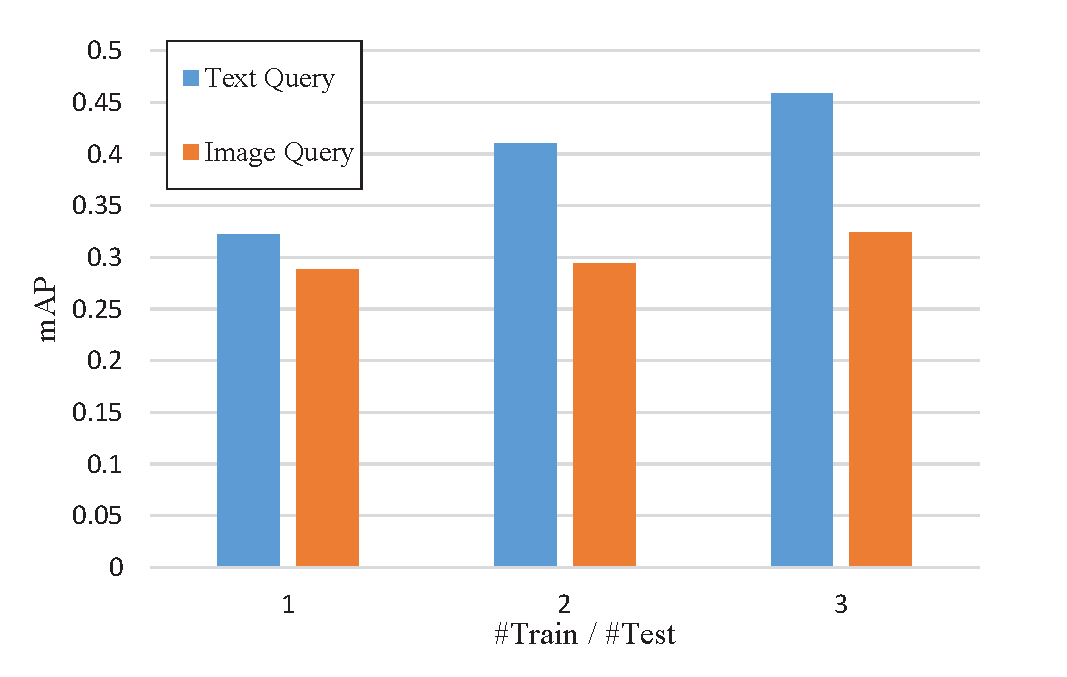
\includegraphics[width=2in]{./fig/train-test-2.eps}%
  \label{fig:train-test-wiki2}}
  \hfil
  \subfloat[NUS-WIDE]{\includegraphics[width=2in]{./fig/train-test-3.eps}%
  \label{fig:train-test-nuswide}}
  \caption{The mAP values obtained by different proportion of training data and test data, on the Wiki and NUS-WIDE datasets, respectively.}
  \label{fig:train-test}
\end{figure*}


Fig.~\ref{fig:paper-fig} shows two examples of our method and other two methods, for image-query-text task and text-query-image task on Wiki dataset, respectively. \textcolor{blue}{Because the text is usually long and it is not easy to get the point, }for image-query-text task, the corresponding images for the top returned texts are shown just for the conveniences of comparison. As illustrated in Fig.~\ref{fig:paper-fig}, for image-query-text task, the query is an image from ``sports'' class. The first three results of our method are relevant. But two of the results of SLiM$^2$ are from other classes and the BLM method returns a irrelevant result firstly. For text-query-image task, the query is a text paragraph on ``biology'' topic that introduces a kind of ``dinosaur''. The returned results of our method are from ``biology'' class, and all of them match the ``dinosaur'' topic obviously, while three results in BLM are irrelevant to the query. The results shown in Fig.~\ref{fig:paper-fig} also prove that our proposed method is effective to the cross-modal retrieval task, and our method outperforms other methods.

\begin{table}[!t]
  \centering
  \caption{\textcolor{blue}{Training and testing time required by our method.}}
  \begin{tabular}{|c|c|c|c|}
  \hline

  Stage& \tabincell{c}{Wiki \\500-D\&1000-D}& \tabincell{c}{Wiki \\1000-D\&5000-D} & NUS-WIDE\\
  \hline
  Training (s)  & 23.65	& 80.65 &	11.79\\
  Testing (s)  & 0.90	& 1.65 &	0.61\\
  \hline
  \end{tabular}
  \label{tab:time}
\end{table}


\textcolor{blue}{In Table \ref{tab:time}, we report the actual training time and testing (retrieval) time required by this approach under the environment of Intel(R) i5-3470 CPU @3.20 GHz and 8G RAM.} Moreover, we change the partitions of the training data and report the performance in the Fig.~\ref{fig:train-test}. As shown in Fig.~\ref{fig:train-test}, the whole performance have a tendency to grow over the scale of training data.



